\documentclass[12pt, letterpaper]{article}

\input{C:/Users/MarEichler17/Documents/MYE-Documents/SCHOOL/Northwestern/preamble}
 



 %line spacing
 \usepackage{setspace}
 \setstretch{1.2}
 
 %header, pagestyle
 \geometry{pass, letterpaper}
 \pagestyle{fancy}
 \fancyhf{} % sets both header and footer to nothing
 \renewcommand{\headrulewidth}{0pt}
 \lhead{STAT 455 Fall 2019 \\ Homework 01}
 \rhead{Martha Eichlersmith \\ Page \thepage \text{ of} \pageref{LastPage}}
 \setlength{\headsep}{48pt}
 \renewcommand{\sectionmark}[1]{\gdef\currsection{\thesection \ #1}}
 \renewcommand{\subsectionmark}[1]{\markright{\currsection\ $\mid$ \thesubsection \  #1}}



\begin{document}
\subsection*{Problem 1}
\subsubsection*{Problem 1a}
$\Xb_i = (X_{i1}, \cdots, X_{id})$  for $i = 1, \cdots, k$\\
$(\Xb_1, \cdots, \Xb_k) \sim \text{Multinomial}(n, \pib_1, \cdots, \pib_k)$ where $\pib_i = (\pi_{i1}, \cdots \pi_{id})$

We know that if $\Yb \sim \text{Multinomial}(n, \pib)$ then the $M_{\Yb}(\tb) = \Ex{ e^{\tb^T \Yb}} = \left( \sum_{i=1}^k \pi_i e^{t_i} \right)^n$.  

Let $\Yb^* = (X_{1+}, \cdots, X_{k+})$ and let  $\tb^* = \begin{bmatrix} 
t_1 & t_2 & \cdots& t_k \\
\vdots & & & \\
t_1 & t_2 & \cdots& t_k 
\end{bmatrix}_{d \times k}$ 
\begin{align*}
M_{\Yb^*}(\tb^*) & = \Ex{ \exp\{(\tb^*)^T \Yb^*\}}
\\
& =  \left( \sum_{i=1}^k \sum_{j=1}^d \pi_{ij} e^{t_{ij}} \right)^n 
\\[0.5ex]
& = \left( \sum_{i=1}^k e^{t_i} \sum_{j=1}^d \pi_{ij} \right)^n & t_{ij} = t_i 
\\[0.5ex]
& = \left( \sum_{i=1}^k e^{t_i} \pi_{i+} \right)^n & \sim \text{Multinomial}(n, \pi_{1+}, \cdots, \pi_{k+})
\end{align*}

\newpage 
\subsubsection*{Problem 1b}
Let $\Yb^* = (Y_a, Y_b, Y_c)$ where $Y_a = X_1 + X_3, \ Y_b = X_2, \ Y_c = X_4 + X_5$ and 
\begin{align*}
M_{\Yb^*}(\tb) & = \Ex{ \exp\{ \tb^T \Yb^* \}}
\\
& = \Ex{ \exp \{ \tb^T(Y_a + Y_b + Y_c)	\}}
\\
& = \Ex{ \exp \{ \tb^T X_1 + \tb^T X_3 + \tb^T X_2 + \tb^T X_4 + \tb^T X_5 \}}
\\
& = \Ex{ \prod_{i=1}^k \exp \{ \tb^T X_i \} } 
\\
& = \prod_{i=1}^n \Ex{ \exp \{ \tb^T X_i \}}
\\
& = \prod_{i=1}^n M_{X_i}(t) 
\\
& = \left( \sum_{j=1}^k \pi_j e^{t_j} \right)^n 
\\[0.5ex]
& \sim \text{Multinomial}(n, \pi_1 + \pi_3, \pi_2, \pi_4 + \pi_5, \ssum_{j=1}^5 \pi_j \leq 1)
\end{align*}

Since $\ssum_{j=1}^6 \pi_j = 1$ we have $\ssum_{j=1}^5 \pi_j \leq 1$.  

\newpage 
\subsubsection*{Problem 1c}
\begin{align*}
\text{Let } Y & = F_X(X) \quad \text{and} \quad U \sim \text{Uniform}(0, 1) 
\\
F_X(x) &= \pr(X \leq x) = 
\begin{cases} 
p_1 & \ \ \  \quad \quad \  x < b_1 \\
p_2 &\ \ \  b_1 \leq x < b_2 \\
\vdots \\
p_k & b_{k-1} \leq x < b_k \\
\vdots \\
p_j & b_j \ \ \ \leq x 
\end{cases} 
\\[2ex]
\omit\rlap{Want to show: $F_Y(y)  \leq \pr(U \leq y) = y \ \forall \ 0 < y < 1$} \\
F_Y(y) & = \pr( Y \leq y) 
\\
& = \pr( F_X(x) \leq y) \quad \quad \text{ Let $p_k \leq  y < p_{k+1}$} 
\\
& = \pr( x_k \leq x < x_{k+1}) = p_k \leq y 
\\
\omit\rlap{Want to show: $F_Y(y)  < \pr(U \leq y) = y  \text{ for some } 0 < y < 1$}  \\
F_Y(y) & = \pr( Y \leq y) 
\\
& = \pr( F_X(x) \leq y) \quad \quad \text{ Let $p_k <  y < p_{k+1}$} 
\\
& = \pr( x_k \leq x < x_{k+1}) = p_k < y 
\end{align*}

\begin{figure}[h]
	\begin{center}
		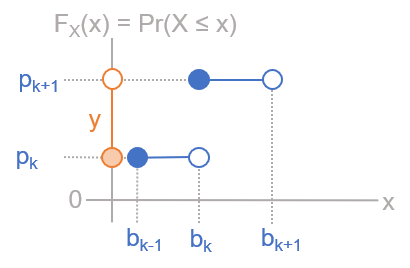
\includegraphics[width=0.48\textwidth]{Fig01c}
	\end{center}
\end{figure}


\subsection*{Problem {\#}1.7} 
\subsubsection*{Problem {\#}1.7.a}  
\begin{align*}
L(\pi) & = \prod_{i=1}^n \pi^{y_i} \cdot (1 - \pi)^{1 - y_i} 
\\
\ell(\pi) & = \left( \ssum_{i=1}^n y_i \right) \log \pi + \left( \ssum_{i=1}^n (1 - y_i) \right) \log (1 - \pi) 
\\[0.5ex]
\frac{ \partial \ell(\pi) }{\partial \pi} 
& = \frac{ \sum_{i=1}^n y_i }{\pi} + \frac{ \ssum_{i=1}^n (1 - y_i) }{1 - pi} \set 0 
\\[0.5ex]
\implies  \ssum_{i=1}^n y_i - \pi \ssum_{i=1}^n y_i & = \pi \ssum_{i=1}^n (1 - y_i) 
\\
\ssum_{i=1}^n y_i & = \pi \underbrace{ \left( \ssum_{i=1}^n (1 - y_i) + \ssum_{i=1}^n y_i \right)}_{ = n} 
\\
\hat{\pi} & = \frac{1}{n} \ssum_{i=1}^n y_i 
\\[0.5ex]
\hat{\pi} & = \frac{1}{20} \cdot 20  = 1 
\end{align*}

\subsubsection*{Problem {\#}1.7.b} 
\begin{align*}
\omit\rlap{Wald Statistics:} \\
W^2 & = \frac{ n \left( \hat{\pi} - \pi_0 \right)^2 }{ \hat{\pi} (1 - \hat{\pi})} 
\\[0.5ex]
& = \frac{ 20 \cdot ( 1 - 0.5)^2}{1 \cdot (1 - 1) } = \frac{5}{0} \quad \text{DNE}, \ \infty 
\\ \quad \\
\omit\rlap{Wald CI:} \\
\hat{\pi} & \pm z_{.025} \sqrt{ \hat{\pi}(1 - \hat{\pi}) / n } \\
1 & \pm 1.96 \cdot 0 \\
\implies & \text{Wald CI: } [1, 1] 
\end{align*}
This is not sensible to use since we are given values that we cannot quantify (i.e. in order to find $\hat{\pi}$, dividing by zero).  


\subsubsection*{Problem {\#}1.7.c}
\begin{tabular}{c c c c}
$S^2$ & $S$ & apval & CI \\ \hline 
20 & 4.4721 & $<$0.0001 & [0.8389, 1]
\end{tabular}
 
\subsubsection*{Problem {\#}1.7.d} 
\begin{tabular}{c c  c}
	$L^2$ & $L$ & CI \\ \hline 
	27.7259 & 5.2655  & [0.9084, 1]
\end{tabular}
\subsubsection*{Problem {\#}1.7.e} 
CP Confidence Interval: [0.8316, 1]  and pval $<$ 0.0001 
\subsubsection*{Problem {\#}1.7.f} 
\begin{align*}
z_{\alpha/2} &= \frac{\hat{\pi} - \pi_T}{ \sqrt{ \pi_T(1 - \pi_T) / n}} 
\\[0.5ex]
n & = \frac{ z_a^2 \pi_T (1 - \pi_T) }{ (\hat{\pi} - \pi_T)^2} 
\\[0.5ex]
n & = 138.2925
\end{align*}
A sample size of 138 is needed.  

\subsection*{Problem {\#}1.8} 
$H_0: \pi_G = 0.75 \vs H_1: \pi_G \neq 0.75$ 

$\hat{\pi}_G = 0.7743$ 

$Z = 1.8601$   

apval $= 0.0629$  

Wald CI: [0.7496, 0.7989]  

Using the traditional threshold of 0.05, we would not reject the null that $\pi_G = 0.75$ (i.e. that the ratio of Green to Yellow is $3:1$).  


\end{document}



%  \text{\textcolor{red}{$$}}
%  \text{\textcolor{blue}{$$}}
%  \text{\textcolor{Green}{$$}}